\section{Introduction} \label{intro}
Functional programming is an increasingly popular paradigm, from its inception in 1950 with Lisp, it was identified as an important paradigm for creating robust, testable, and scalable code \cite{whyfunctional}. The 2015 review of Hughes' article by Hu et al. \cite{howfunctional} highlighted the explosion of functional features, especially higher order functions, in modern languages such as C\#, C++, and Java, as well as how further research has led to improved performance of lazy evaluation. Other features, such as lazy evaluation (seen in Python's generator functions), have been slower to uptake despite potential benefits. 

When looking at what functional programmers practice, it's no wonder why it's grown as a paradigm so much. The focus on pure functions (those without side effects, depending entirely on their inputs), and immutable data allows a programmer to write testable, reliable code, and may be the key to efficient parallel processing\cite{swaine2008s}. A focus on these practices can lead to more maintainable code, with guarantees that changes to how a function works (of course, assuming the changes are correct) won't affect other functions at all, greatly reducing the complexity of a code base.

It is no surprise that this has also led to a rise in functional programming within both online and university courses \cite{warwickFP, kentFP, birminghamFP, courseraFP}, but the barrier to entry is still high. Singer and Archibald's 2018 paper \cite{singer2018functional}, which analysed 161,000 interactions from over 3,000 Haskell learners, found around 3\% of lines contained syntax errors, and 18\% of syntactically correct expressions contained type errors.

\subsection{Haskell Visualiser}
The aim of this project has been a Haskell Visualiser, example are shown in Figure \ref{fig:broad-example}. Being able to see the expression, subsets of the expression, and their types makes it easier to understand. This enables the user to know why their expression is or is not well-typed, and changes to the expression are quickly realised for fast debugging. A number of preset examples exist, to show the syntax, what features of the Haskell language are implemented, and how they work.
\begin{figure}
    \centering
    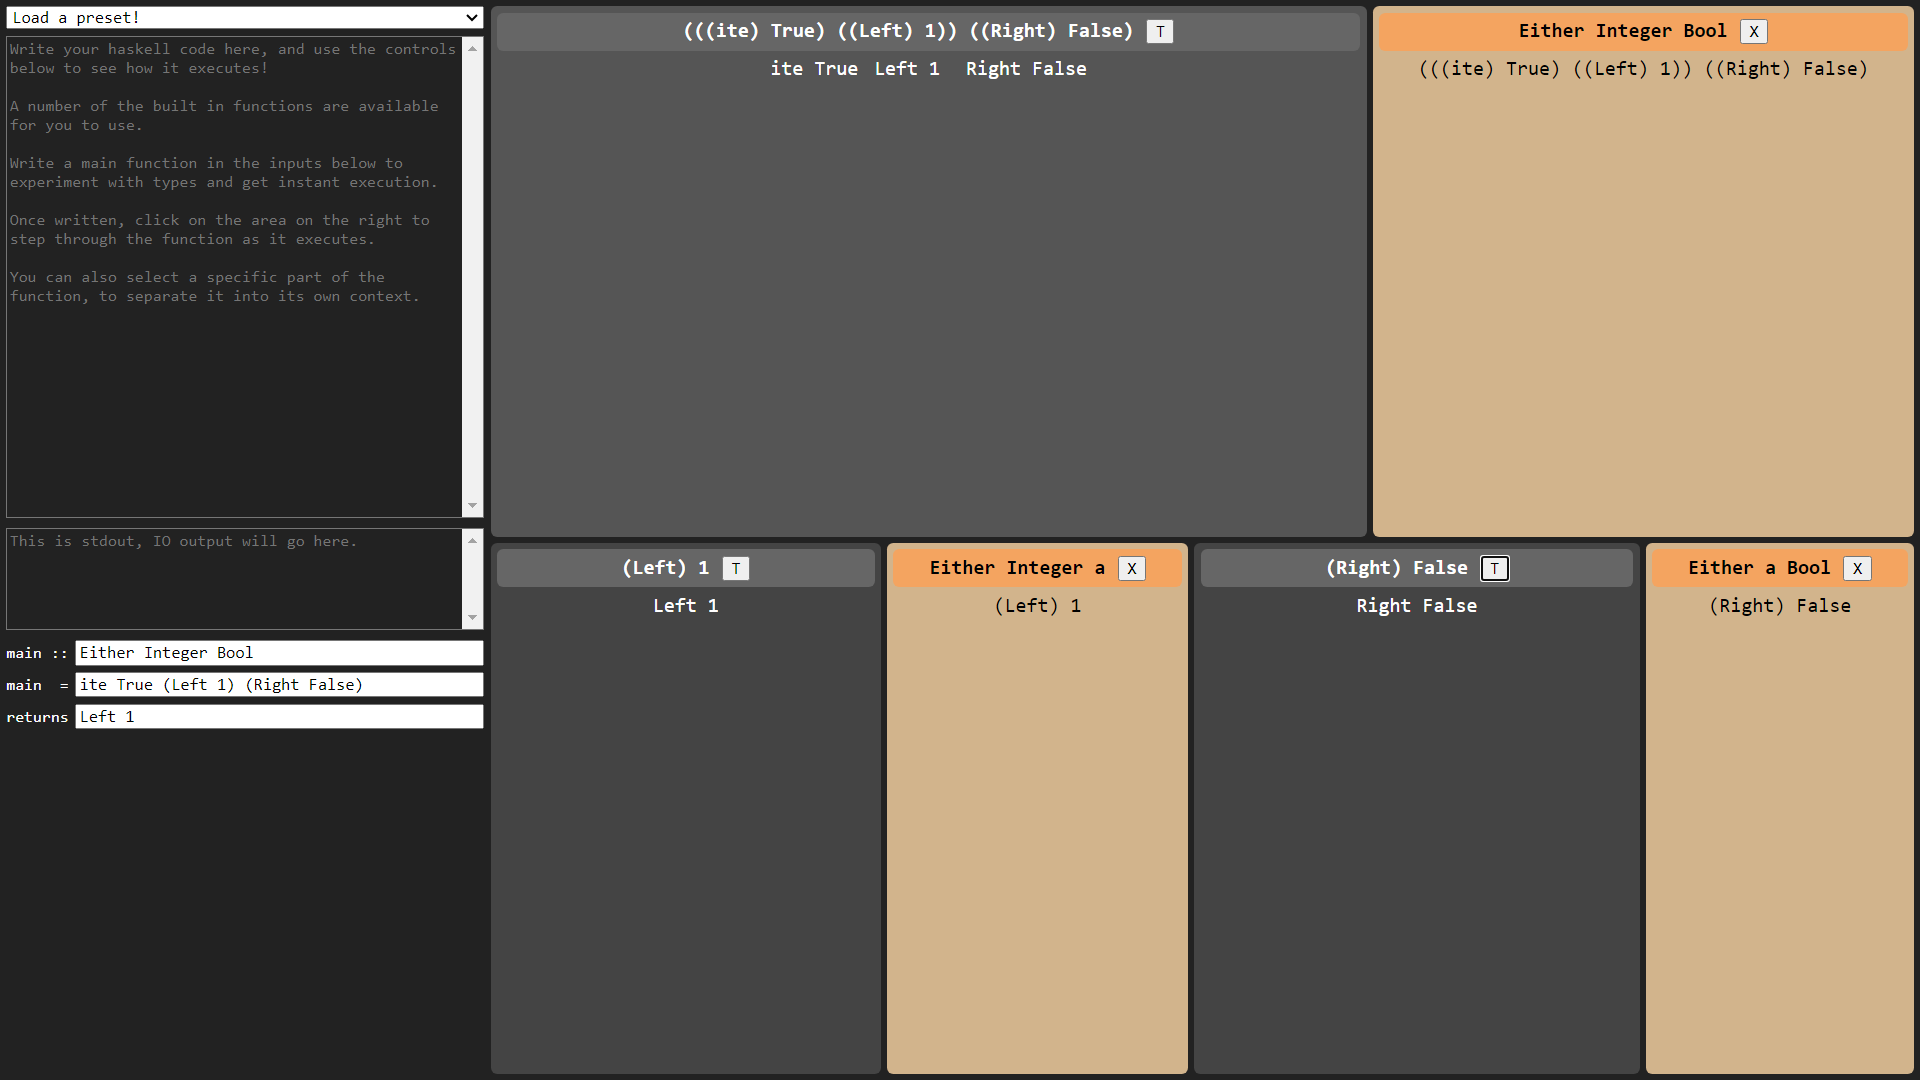
\includegraphics[width=1\linewidth]{chapters//1-introduction//resources/example.png}
    \caption{The Haskell Visualiser, showing the term ``ite True (Left 1) (Right 'a')'', and some type information.}
    \label{fig:broad-example}
\end{figure}

This has been implemented with a custom programming language covering a subset of the Haskell syntax, who's grammar is described in Section \ref{syntax}. This language supports polymorphic functions, custom data types, and function overloading through type classes, and is capable of inferring the type of expressions as they evaluate. As the aim was to lower the barrier to entry, a subset of the standard library has also been implemented for use in user's functions.

\subsection{Report Structure}
Section \ref{background} provides the required background knowledge. Section \ref{specification} contains the specification, detailing what the project requires to be a success. Section \ref{design} goes over the what and why of the design decisions, and Section \ref{implementation} details how that design were implemented. Section \ref{testing} covers the testing, and Section \ref{evaluation} describes the outcome of the project. Lastly, Section \ref{conclusion} evaluates the overall outcome of the project.